\documentclass[11pt]{article}

\usepackage[left=2.5cm, right=2cm, top=0.6cm, bottom=2cm, includehead, includefoot]{geometry}
\usepackage[utf8]{inputenc}
\usepackage[T1]{fontenc}
\usepackage{titlesec}
\usepackage{enumitem}
\usepackage{graphicx}
\usepackage{amsmath}
\usepackage{amsfonts}
\usepackage{amssymb}
\usepackage{parskip}
\usepackage{float}
\usepackage{setspace}
\usepackage{fancyhdr}
\usepackage{needspace}
\usepackage{etoolbox}
\usepackage{url}
\usepackage{placeins}
\usepackage{tikz}
\usetikzlibrary{arrows.meta, positioning}

\newcommand{\figpendiente}[2]{
    \fbox{
        \begin{minipage}[c][3.4cm][c]{0.88\textwidth}
            \centering
            \textbf{Figura pendiente}\\[0.4em]
            #1\\[0.4em]
            {\footnotesize #2}
        \end{minipage}
    }
}

\pagestyle{fancy}
\fancyhf{}
\setlength{\headheight}{63pt}
\setlength{\headsep}{10pt}
\fancyhead[L]{}
\fancyhead[R]{}
\fancyhead[C]{} % \includegraphics[width=\textwidth]{picture/logo.pdf} si existe
\renewcommand{\headrulewidth}{0pt}
\fancyfoot[C]{\thepage}
\setlength{\footskip}{18pt}

\setstretch{1.12}
\setlength{\parskip}{0.65em}
\setlist[itemize]{leftmargin=1.35cm, itemsep=0.45em, topsep=0.35em}
\setlist[enumerate]{leftmargin=1.35cm, itemsep=0.45em, topsep=0.35em}

\titleformat{\section}{\normalfont\Large\bfseries}{\thesection}{1em}{}
\titleformat{\subsection}{\normalfont\large\bfseries}{\thesubsection}{1em}{}
\preto{\subsection}{\Needspace{10\baselineskip}}
\preto{\subsubsection}{\Needspace{8\baselineskip}}
\preto{\subsection}{\FloatBarrier}
\preto{\subsubsection}{\FloatBarrier}

\title{Informe del Proyecto}
\raggedbottom

\begin{document}

\renewcommand{\figurename}{Figura}
\renewcommand{\thesection}{\Roman{section}}
\begin{center}
    \textbf{\underline{\normalsize APE 1}}
\end{center}

\section{PORTADA}

\begin{tabbing}
    \textbf{Unidad de Organización Curricular:}\hspace{1cm} \= \kill
    \textbf{Tema:} \> Procesamiento de Imágenes en Dominio Espacial y Frecuencia \\[0.25em]
    \textbf{Carrera:} \> Ingeniería de Software \\[0.25em]
    \textbf{Unidad de Organización Curricular:} \> PROFESIONAL \\[0.25em]
    \textbf{Nivel y Paralelo:} \> Séptimo A \\[0.25em]
    \textbf{Alumnos participantes:} \> Paul Velastegui \\
    \> David Manjarres \\[0.25em]
    \textbf{Asignatura:} \> Inteligencia Artificial \\[0.25em]
    \textbf{Docente:} \> Ing. Rubén Nogales, Mg.
\end{tabbing}

\section{INFORME DE GUÍA PRÁCTICA}
\renewcommand{\thesection}{\arabic{section}}

\subsection{Objetivos}
\textbf{General:}
\begin{itemize}
    \item Desarrollar y documentar una aplicación de escritorio para el procesamiento digital de imágenes orientada al análisis de placas vehiculares, integrando preprocesamiento, suavizado, acentuado, binarización, detección de bordes, segmentación por regiones y extracción de submatrices.
\end{itemize}

\textbf{Específicos:}
\begin{itemize}
    \item Implementar manualmente algoritmos de conversión a grises, ecualización de histograma, ruido sal y pimienta, filtros de media, mediana, moda, operadores de acentuado y detección de bordes.
    \item Comparar el comportamiento de filtros espaciales y frecuenciales, diferenciando su efecto sobre ruido, detalle fino, bordes y segmentación posterior.
    \item Aplicar operadores de gradiente como Roberts, Prewitt, Sobel, Kirsch y Laplaciano para analizar su utilidad en la detección de caracteres de placas.
    \item Construir una etapa de detección de regiones mediante BFS, filtrando por forma, tamaño y posición antes de generar submatrices normalizadas.
\end{itemize}

\subsection{Modalidad}
\begin{tabbing}
    \hspace{1cm} \= Virtual.
\end{tabbing}

\subsection{Tiempo de duración}
\begin{tabbing}
    \hspace{1cm} \= \textbf{Presenciales:} \= 8 \\
    \hspace{1cm} \= \textbf{No presenciales:} \= 0
\end{tabbing}

\subsection{Instrucciones}
\begin{enumerate}
    \item Cargar una imagen desde la interfaz gráfica.
    \item Ajustar el porcentaje de ruido Sal y Pimienta para simular degradación impulsiva.
    \item Seleccionar el filtro de suavizado, su dominio de trabajo y el tamaño de máscara o frecuencia de corte $D_0$.
    \item Seleccionar el tipo de acentuado espacial o frecuencial que resaltará bordes antes de la binarización.
    \item Definir el umbral de binarización, el operador de gradiente y los rangos de área para la detección de regiones.
    \item Revisar secuencialmente las pestañas Escala de grises, Suavizado, Acentuado, Binarización, Gradiente y Regiones.
\end{enumerate}

\subsection{Listado de equipos, materiales y recursos}
\begin{itemize}
    \item Computador con Python 3 instalado.
    \item Imágenes digitales de prueba en formato estándar (\texttt{png}, \texttt{jpg}, \texttt{jpeg}).
    \item Entorno virtual con las dependencias del proyecto.
\end{itemize}

\subsubsection*{Dependencias de Python utilizadas}
\begin{itemize}
    \item \textbf{OpenCV:} Utilizado de forma exclusiva para lectura/escritura de archivos y decodificación. \textit{Se prohibió explícitamente} el uso de funciones como \texttt{cv2.filter2D} o \texttt{imnoise}.
    \item \textbf{NumPy:} Empleado para la manipulación de matrices multidimensionales y para realizar la transformada rápida de Fourier (\texttt{np.fft.fft2}).
    \item \textbf{PySide6:} Herramienta de interfaz gráfica (GUI) que estructura la visualización mediante pestañas, \textit{sliders} y cuadros combinados.
    \item \textbf{Matplotlib:} Usado mediante su \textit{backend} integrado en PySide6 para visualizar de manera comparativa las diferentes salidas (espectros, mapas de color e imágenes RGB).
\end{itemize}

\textbf{TAC (Tecnologías para el Aprendizaje y Conocimiento) empleados en la guía práctica:}

$\square$ Plataformas educativas \\
$\square$ Simuladores y laboratorios virtuales \\
$\blacksquare$ Aplicaciones educativas \\
$\square$ Recursos audiovisuales \\
$\square$ Gamificación \\
$\blacksquare$ Inteligencia Artificial \\
Otros (Especifique): \underline{\hspace{5cm}}

\subsection{Actividades por desarrollar}
\begin{enumerate}
    \item Diseñar una arquitectura de software dividida en interfaz (\texttt{interfaz.py}) y lógica algorítmica (\texttt{modelo.py}).
    \item Programar el flujo de conversión a grises y normalización de histograma con recorridos manuales.
    \item Construir los bucles anidados para la convolución discreta en $2D$ garantizando el \textit{padding}.
    \item Implementar la inserción secuencial (\textit{Insertion Sort}) para el filtro de mediana, y diccionarios para contar frecuencias en el filtro de moda, evadiendo funciones preconstruidas.
    \item Implementar operadores de acentuado y gradiente con máscaras manuales, incluyendo componentes direccionales.
    \item Implementar segmentación por regiones conexas usando BFS, filtrado de regiones no útiles y extracción de submatrices.
    \item Establecer un procesamiento asíncrono (\textit{Worker Threads}) para no bloquear la GUI durante los cálculos cíclicos en Python.
\end{enumerate}

\subsection{Resultados obtenidos}

El sistema desarrollado no se limita a aplicar un filtro aislado. La aplicación propone una cadena completa de procesamiento: conversión a escala de grises, normalización, inserción controlada de ruido, suavizado, acentuado, binarización, gradiente, limpieza de máscara, detección de regiones y extracción de submatrices. Este orden permite observar cómo una decisión temprana, como el tipo de suavizado, modifica directamente el comportamiento del \textit{bounding box} final.

El criterio de implementación fue mantener los algoritmos principales visibles en el código. NumPy se utilizó como contenedor de matrices y para la FFT, mientras que las operaciones centrales de la práctica se resolvieron con recorridos explícitos: conteo de histograma, convolución, ordenamiento de mediana, moda, binarización, gradientes, BFS y redimensionamiento de submatrices.

\subsubsection{Flujo general del sistema}

La Figura \ref{fig:flujo_general} resume el recorrido de una placa dentro del sistema. La imagen se normaliza y degrada con ruido sal y pimienta para probar la robustez de los filtros. Luego se suaviza, se acentúa, se binariza y se somete a un operador de gradiente. Finalmente, el mapa de bordes se limpia antes de buscar regiones conexas y generar submatrices normalizadas.

\begin{figure}[H]
    \centering
    \begin{tikzpicture}[
        node distance=0.7cm,
        etapa/.style={draw, rounded corners, align=center, minimum width=2.4cm, minimum height=0.75cm, fill=blue!6},
        flecha/.style={-{Latex[length=2mm]}, thick}
    ]
        \node[etapa] (a) {Imagen\\original};
        \node[etapa, right=of a] (b) {Grises +\\normalización};
        \node[etapa, right=of b] (c) {Ruido +\\suavizado};
        \node[etapa, below=of c] (d) {Acentuado};
        \node[etapa, left=of d] (e) {Binarización};
        \node[etapa, left=of e] (f) {Gradiente};
        \node[etapa, below=of f] (g) {Limpieza\\de máscara};
        \node[etapa, right=of g] (h) {BFS +\\filtros};
        \node[etapa, right=of h] (i) {Bounding boxes\\y recortes};
        \draw[flecha] (a) -- (b);
        \draw[flecha] (b) -- (c);
        \draw[flecha] (c) -- (d);
        \draw[flecha] (d) -- (e);
        \draw[flecha] (e) -- (f);
        \draw[flecha] (f) -- (g);
        \draw[flecha] (g) -- (h);
        \draw[flecha] (h) -- (i);
    \end{tikzpicture}
    \caption{Flujo general aplicado para preparar una placa vehicular antes de extraer regiones candidatas.}
    \label{fig:flujo_general}
    \vspace{2pt}
    {\footnotesize Fuente: Elaboración propia.}
\end{figure}

\subsubsection{Preprocesamiento: escala de grises y normalización}

La conversión a escala de grises se implementó con la ponderación perceptiva BT.601:

\begin{equation}
    I_{gris}(x,y)=0.299R+0.587G+0.114B
\end{equation}

Posteriormente se aplicó ecualización de histograma mediante el cálculo manual de frecuencias y de la función de distribución acumulada. Esta etapa ayuda a que placas con iluminación irregular tengan un contraste más aprovechable antes de binarizar.

\begin{figure}[H]
    \centering
    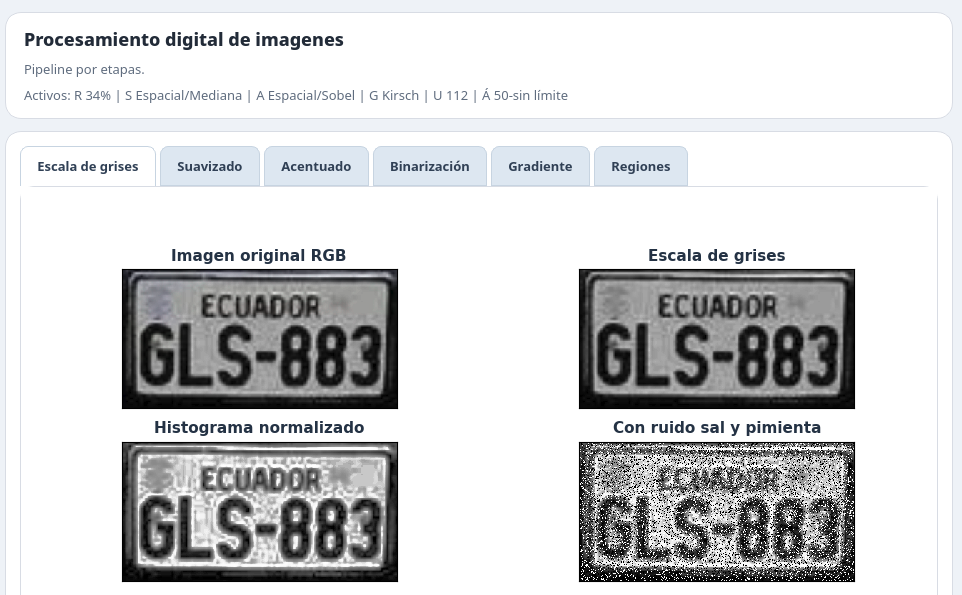
\includegraphics[width=0.85\textwidth]{img/escala-grises.png}
    \caption{Conversión inicial de la imagen a escala de grises y preparación tonal para las etapas posteriores.}
    \label{fig:escala_grises}
    \vspace{2pt}
    {\footnotesize Fuente: Elaboración propia.}
\end{figure}

\subsubsection{Ruido y suavizado espacial}

Se introdujo ruido sal y pimienta para comprobar si los filtros espaciales podían recuperar estructura útil sin destruir los caracteres. El ruido se agregó seleccionando posiciones aleatorias y sustituyendo sus valores por 0 o 255.

\textbf{Filtro de media:} promedia la vecindad $N \times N$. Reduce variaciones locales, pero puede difuminar bordes de letras y números.

\textbf{Filtro de mediana:} ordena manualmente los valores de la vecindad y toma el elemento central. Fue el filtro más conveniente para ruido sal y pimienta porque elimina impulsos aislados sin promediar todos los contornos.

\textbf{Filtro de moda:} selecciona el valor más repetido dentro de la máscara. Es útil cuando predominan intensidades repetidas, aunque puede ser menos estable en zonas con textura o degradación fotográfica.

\begin{table}[H]
    \centering
    \renewcommand{\arraystretch}{1.25}
    \begin{tabular}{|p{3.1cm}|p{4.2cm}|p{4.2cm}|p{3.1cm}|}
        \hline
        \textbf{Filtro} & \textbf{Ventaja observada} & \textbf{Riesgo observado} & \textbf{Uso recomendado} \\
        \hline
        Media & Suaviza ruido distribuido y pequeñas variaciones. & Puede borrar bordes finos de caracteres. & Imágenes con ruido suave. \\
        \hline
        Mediana & Elimina puntos sal y pimienta conservando mejor la forma. & Con máscaras grandes puede deformar trazos delgados. & Placas con ruido impulsivo. \\
        \hline
        Moda & Conserva valores dominantes en una vecindad. & Puede generar bloques duros si la imagen no es casi binaria. & Máscaras binarias o zonas uniformes. \\
        \hline
    \end{tabular}
    \caption{Comparación cualitativa de filtros espaciales implementados manualmente.}
    \label{tab:comparacion_suavizado}
\end{table}

\begin{figure}[H]
    \centering
    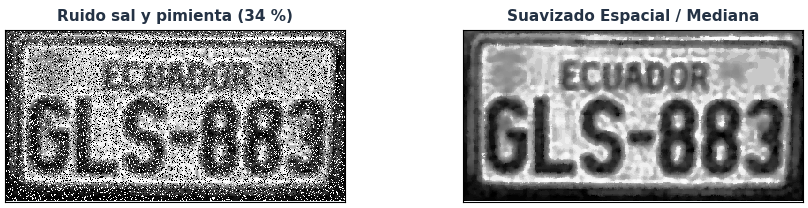
\includegraphics[width=0.9\textwidth]{img/suavizado.png}
    \caption{Comparación entre la imagen con ruido y la imagen suavizada. La mediana preserva mejor los bordes principales cuando el ruido es impulsivo.}
    \label{fig:suavizado}
    \vspace{2pt}
    {\footnotesize Fuente: Elaboración propia.}
\end{figure}

% IMAGEN PENDIENTE: capturar desde la pestaña "Suavizado" tres ejecuciones de la misma placa: Media 5x5, Mediana 5x5 y Moda 5x5. Guardar como img/comparacion-suavizados.png. Conviene usar el mismo porcentaje de ruido y explicar que la comparación es justa porque cambia solo el filtro.
\begin{figure}[H]
    \centering
    \figpendiente{Comparación visual entre Media, Mediana y Moda con la misma máscara.}{Obtención: ejecutar la app tres veces con igual imagen, ruido y máscara; cambiar únicamente el filtro de suavizado.}
    \caption{Figura propuesta para comparar la respuesta de los filtros espaciales ante ruido sal y pimienta.}
    \label{fig:comparacion_suavizados}
\end{figure}

\subsubsection{Acentuado espacial y frecuencial}

El acentuado se ubicó después del suavizado porque una imagen suavizada tiene menos ruido aislado y permite resaltar bordes con menor riesgo de amplificar puntos falsos. En dominio espacial se emplearon operadores como Roberts, Prewitt, Sobel y Laplaciano. En dominio frecuencial se aplicó un filtro pasa-altas gaussiano controlado por $D_0$.

En el caso de placas, Sobel fue una opción equilibrada para el acentuado espacial: detecta cambios horizontales y verticales con mayor estabilidad que Roberts y sin la agresividad direccional de Kirsch. Esto deja letras y números más marcados antes del umbral.

\begin{figure}[H]
    \centering
    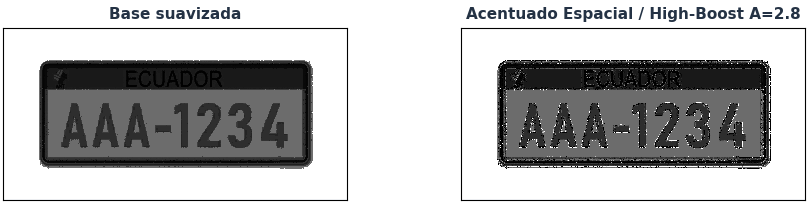
\includegraphics[width=0.9\textwidth]{img/acentuado.png}
    \caption{Resultado de la etapa de acentuado. Esta fase mejora la separación visual de caracteres antes de binarizar.}
    \label{fig:acentuado}
    \vspace{2pt}
    {\footnotesize Fuente: Elaboración propia.}
\end{figure}

% IMAGEN PENDIENTE: capturar la pestaña "Acentuado" comparando Roberts, Sobel y Laplaciano sobre la misma placa suavizada. Guardar como img/comparacion-acentuado.png. Interpretar Sobel como opción estable y Roberts como sensible al ruido.
\begin{figure}[H]
    \centering
    \figpendiente{Comparación de operadores de acentuado espacial.}{Obtención: mantener igual suavizado y umbral; cambiar únicamente el operador de acentuado.}
    \caption{Figura propuesta para justificar la selección del operador de acentuado en placas vehiculares.}
    \label{fig:comparacion_acentuado}
\end{figure}

\subsubsection{Binarización}

La binarización convierte la imagen acentuada en una máscara de dos niveles. En esta etapa el umbral $T$ determina qué píxeles serán considerados parte del objeto:

\begin{equation}
    I_{bin}(x,y)=
    \begin{cases}
        255, & \text{si } I_{acentuada}(x,y)\geq T \\
        0, & \text{si } I_{acentuada}(x,y)<T
    \end{cases}
\end{equation}

Un umbral demasiado bajo conserva ruido y zonas del fondo; uno demasiado alto fragmenta caracteres. Por esta razón, la interfaz mantiene el umbral como parámetro ajustable antes del gradiente y de la detección de regiones.

\begin{figure}[H]
    \centering
    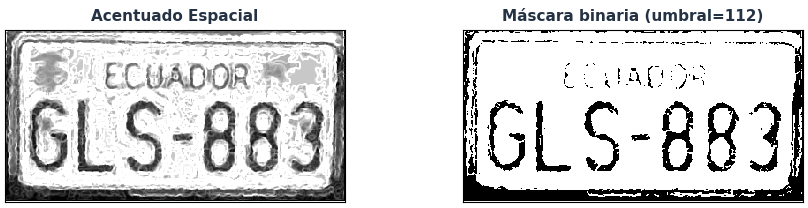
\includegraphics[width=0.85\textwidth]{img/binarizacion.png}
    \caption{Binarización posterior al acentuado. El umbral define la cantidad de información que pasa al detector de bordes.}
    \label{fig:binarizacion}
    \vspace{2pt}
    {\footnotesize Fuente: Elaboración propia.}
\end{figure}

\subsubsection{Gradiente y operadores direccionales}

Después de binarizar se aplica un operador de gradiente para obtener el mapa de bordes. En el proyecto se incluyeron Roberts, Prewitt, Sobel, Kirsch y Laplaciano. Los tres primeros calculan componentes direccionales $G_x$ y $G_y$, mientras que Kirsch evalúa varias direcciones y conserva la respuesta máxima. Laplaciano responde a cambios de segundo orden y no separa explícitamente horizontal/vertical.

\begin{table}[H]
    \centering
    \renewcommand{\arraystretch}{1.25}
    \begin{tabular}{|p{2.8cm}|p{4.2cm}|p{4.5cm}|p{3.2cm}|}
        \hline
        \textbf{Operador} & \textbf{Comportamiento} & \textbf{Interpretación en placas} & \textbf{Recomendación} \\
        \hline
        Roberts & Máscara pequeña, sensible a cambios diagonales. & Detecta bordes rápidos, pero reacciona fuerte al ruido. & Comparación o imágenes limpias. \\
        \hline
        Prewitt & Gradiente 3x3 simple. & Bordes estables, aunque menos marcados que Sobel. & Alternativa académica. \\
        \hline
        Sobel & Pondera más el centro de la máscara. & Buen equilibrio entre borde y ruido. & Opción principal. \\
        \hline
        Kirsch & Evalúa direcciones y toma la máxima respuesta. & Resalta contornos fuertes, útil si los caracteres están débiles. & Prueba secundaria. \\
        \hline
        Laplaciano & Respuesta isotrópica de segundo orden. & Puede marcar bordes y ruido al mismo tiempo. & Experimentación. \\
        \hline
    \end{tabular}
    \caption{Comparación de operadores de gradiente implementados en el sistema.}
    \label{tab:comparacion_gradientes}
\end{table}

\begin{figure}[H]
    \centering
    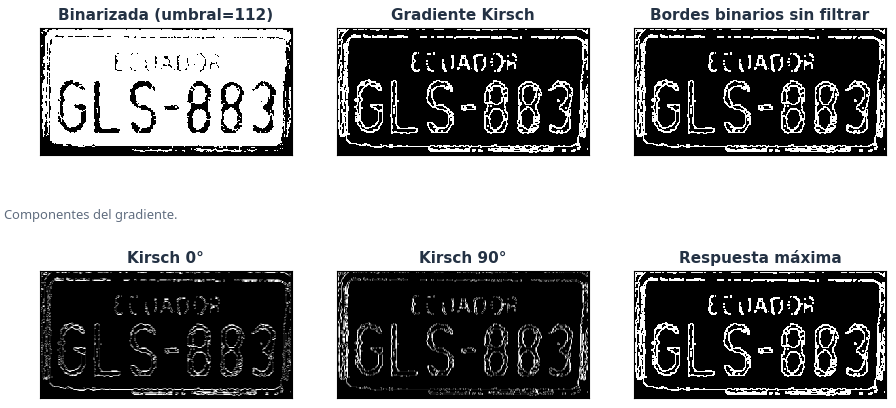
\includegraphics[width=0.9\textwidth]{img/gradiente.png}
    \caption{Visualización del gradiente y sus componentes. Esta etapa genera el mapa de bordes que alimenta la detección de regiones.}
    \label{fig:gradiente}
    \vspace{2pt}
    {\footnotesize Fuente: Elaboración propia.}
\end{figure}

% IMAGEN PENDIENTE: capturar desde la pestaña "Gradiente" una comparación Sobel vs Kirsch usando la misma imagen binarizada. Guardar como img/comparacion-gradientes.png. En la interpretación indicar que Kirsch marca más contornos, pero Sobel puede dejar menos ruido para BFS.
\begin{figure}[H]
    \centering
    \figpendiente{Comparación entre Sobel y Kirsch sobre la misma máscara binaria.}{Obtención: ejecutar dos veces con iguales parámetros previos; cambiar solo el operador de gradiente.}
    \caption{Figura propuesta para comparar estabilidad y fuerza de respuesta de los gradientes.}
    \label{fig:comparacion_gradientes}
\end{figure}

\subsubsection{Detección de regiones, \textit{bounding boxes} y submatrices}

La detección de regiones se realizó sobre la máscara de bordes filtrada. Primero se eliminan puntos aislados verificando que cada píxel blanco tenga vecinos blancos cercanos. Luego se ejecuta BFS con 4-vecindad para agrupar píxeles conectados. Finalmente, cada región se filtra por área, proporción, tamaño y posición vertical.

Esta decisión es importante: el sistema no ``lee'' que un texto dice ECUADOR; lo descarta porque sus regiones suelen ser más pequeñas, estar ubicadas en la zona superior o tener proporciones distintas a los caracteres principales de la placa. De forma similar, el marco de la placa se descarta por ser una región demasiado grande o demasiado ancha.

\begin{figure}[H]
    \centering
    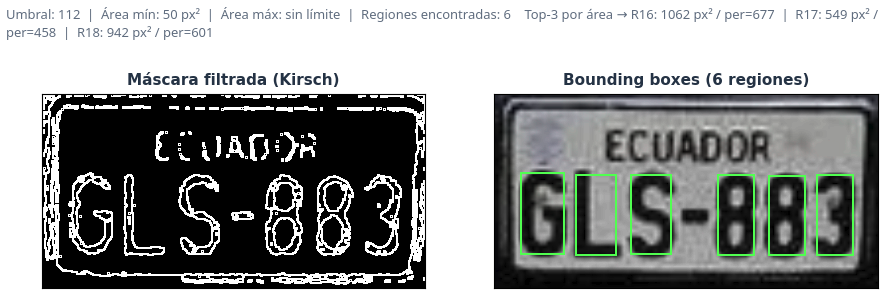
\includegraphics[width=0.9\textwidth]{img/regiones-1.png}
    \caption{Detección de regiones sobre la placa. Los \textit{bounding boxes} se dibujan sobre la imagen original para interpretar visualmente qué objetos fueron aceptados.}
    \label{fig:regiones}
    \vspace{2pt}
    {\footnotesize Fuente: Elaboración propia.}
\end{figure}

\begin{figure}[H]
    \centering
    
\includegraphics[width=0.9\textwidth]{img/regiones-2.png}
    \caption{Submatrices normalizadas. Cada recorte se redimensiona por vecino más cercano para preparar una posible entrada a un clasificador.}
    \label{fig:submatrices}
    \vspace{2pt}
    {\footnotesize Fuente: Elaboración propia.}
\end{figure}

% IMAGEN PENDIENTE: capturar una comparación antes/después del filtrado de regiones. La primera imagen debe mostrar el gradiente binario bruto con muchas regiones; la segunda debe mostrar la máscara filtrada y los bounding boxes finales. Guardar como img/comparacion-regiones.png.
\begin{figure}[H]
    \centering
    \figpendiente{Comparación entre regiones detectadas antes y después del filtrado por forma, tamaño y posición.}{Obtención: capturar la pestaña Gradiente y luego la pestaña Regiones con los mismos parámetros.}
    \caption{Figura propuesta para demostrar que el filtrado reduce ruido, texto superior y marco de placa.}
    \label{fig:comparacion_regiones}
\end{figure}

\subsubsection{El dominio de frecuencia}

El filtrado en frecuencia no trabaja con vecindades de píxeles, sino con componentes senoidales y cosenoidales de la imagen. En el sistema se incluyeron dos opciones: pasa-bajas gaussiano para suavizado frecuencial y pasa-altas gaussiano para acentuado frecuencial. Ambos usan una frecuencia de corte $D_0$ configurable.

El flujo construido consta de:

\begin{enumerate}
    \item Aplicar la Transformada Rápida de Fourier en 2D (\texttt{np.fft.fft2}).
    \item Centrar el espectro de bajas frecuencias en el origen mediante un \textit{shift}.
    \item Construir manualmente una máscara gaussiana iterando sobre cada coordenada $(u, v)$, determinando su distancia al centro y aplicando $e^{-D(u,v)^2/(2D_0^2)}$.
    \item Multiplicar iterativamente el espectro complejo por la máscara real (punto a punto con bucles).
    \item Revertir el espectro al dominio espacial aplicando la Transformada Inversa (IFFT) y normalizando su parte real.
\end{enumerate}

\begin{figure}[htbp]
    \centering
    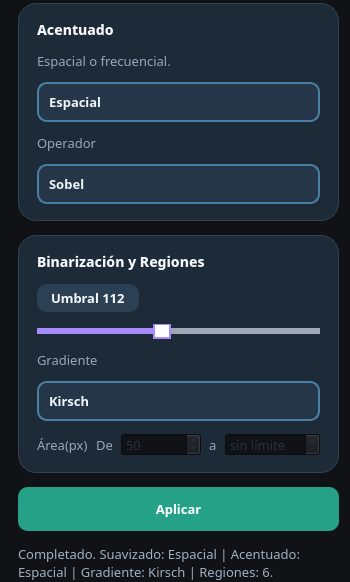
\includegraphics[width=0.82\textwidth,height=0.42\textheight,keepaspectratio]{img/filtros-app-2.png}
    \caption{Diagnóstico en frecuencia. Se observa el espectro original, la máscara gaussiana, el espectro filtrado y la reconstrucción espacial.}
    \label{fig:app_frecuencia}
    \vspace{2pt}
    {\footnotesize Fuente: Elaboración propia.}
\end{figure}

El filtro gaussiano tiene la ventaja de no poseer una frecuencia de corte abrupta, por lo que reduce el riesgo de artefactos de anillado. En suavizado, un $D_0$ menor produce una imagen más borrosa; en acentuado, el pasa-altas resalta bordes y detalles al atenuar las bajas frecuencias.

% IMAGEN PENDIENTE: capturar el mismo suavizado frecuencial con D0 bajo, medio y alto. Guardar como img/comparacion-d0.png. Interpretar cómo cambia el detalle: D0 bajo suaviza más; D0 alto conserva más estructura.
\begin{figure}[htbp]
    \centering
    \figpendiente{Variación del parámetro $D_0$ en el dominio de frecuencia.}{Obtención: seleccionar suavizado frecuencial y ejecutar con tres valores de $D_0$ manteniendo fija la imagen.}
    \caption{Figura propuesta para mostrar la sensibilidad del filtro frecuencial al radio de corte.}
    \label{fig:comparacion_d0}
\end{figure}

\subsubsection{Arquitectura y Experiencia de Usuario}

La interfaz, construida sobre PySide6, soluciona la paralización del sistema (generada por la complejidad de $O(N^2 \cdot M^2)$ de los filtros manuales) mediante el uso de \texttt{QThread}. Esto delega la pesada tarea matemática a núcleos secundarios de la CPU, manteniendo fluida la interacción con las pestañas y visualizaciones.

\begin{figure}[H]
    \centering
    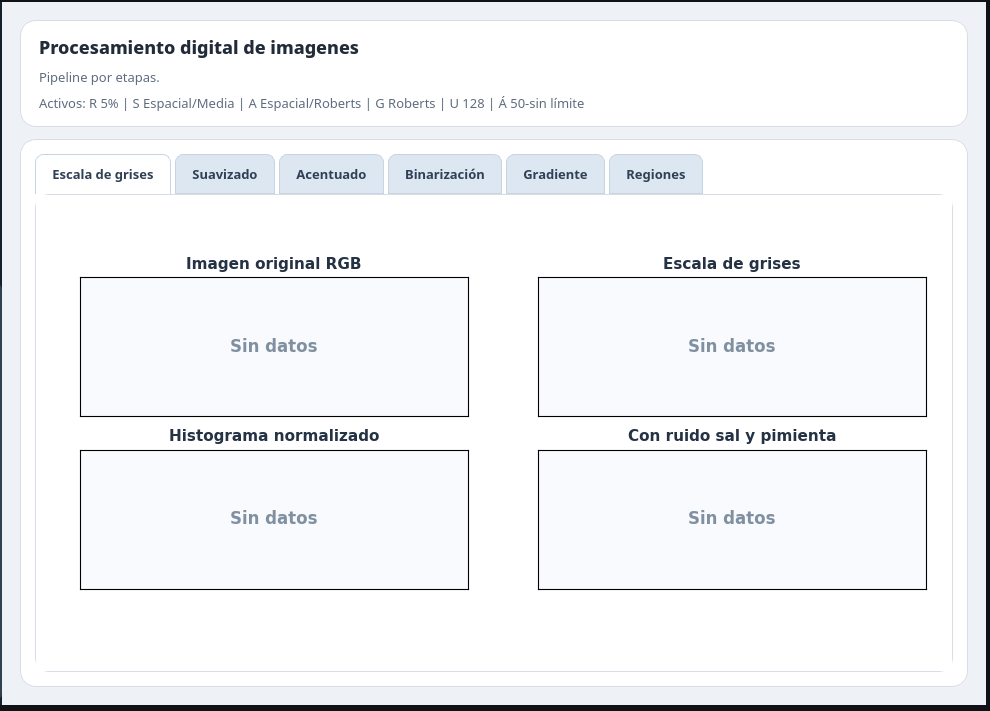
\includegraphics[width=0.95\textwidth]{img/vista-general.png}
    \caption{Vista General de la Interfaz. A la izquierda los paneles de parámetros en tiempo real, a la derecha el visor embebido de Matplotlib Canvas.}
    \label{fig:vista_general}
    \vspace{2pt}
    {\footnotesize Fuente: Elaboración propia.}
\end{figure}

\subsection{Habilidades blandas empleadas en la práctica}
$\blacksquare$ Trabajo en equipo \\
$\square$ Liderazgo \\
$\square$ Comunicación asertiva \\
$\blacksquare$ Responsabilidad \\
$\blacksquare$ Pensamiento crítico \\
$\blacksquare$ Resolución de problemas \\
$\blacksquare$ Adaptabilidad \\
$\square$ Gestión del tiempo \\
$\square$ Resolución de conflictos

\subsection{Conclusiones}

El desarrollo manual de algoritmos de procesamiento de imágenes evidenció la carga computacional que las librerías modernas suelen ocultar. El reemplazo de operaciones optimizadas por bucles secuenciales aumentó los tiempos de procesamiento, pero permitió comprender de forma directa cómo se construyen filtros, máscaras, histogramas, gradientes y regiones conexas.

La separación entre suavizado, acentuado, binarización y gradiente permitió comprobar que la segmentación final depende de toda la cadena, no de un único operador. En placas vehiculares, la mediana resultó adecuada para ruido sal y pimienta, mientras que Sobel ofreció una respuesta estable para resaltar caracteres antes de la binarización.

La detección de regiones demostró que no basta con obtener bordes: también es necesario filtrar componentes por tamaño, forma y posición. Esta etapa permitió descartar ruido, fragmentos del marco y texto superior de la placa, produciendo submatrices más útiles para una futura red neuronal.

El dominio de frecuencia complementó el análisis espacial al mostrar cómo $D_0$ controla el paso o rechazo de frecuencias. El pasa-bajas suaviza globalmente la imagen, mientras que el pasa-altas resalta detalles y bordes. Su interpretación visual mediante espectros permitió relacionar la teoría de Fourier con resultados observables en la interfaz.

\subsection{Recomendaciones}

Para placas con ruido sal y pimienta se recomienda iniciar con suavizado por mediana y máscaras moderadas, por ejemplo $3 \times 3$ o $5 \times 5$. Máscaras grandes pueden limpiar más ruido, pero también deforman trazos delgados de letras y números.

Para acentuado se recomienda utilizar Sobel como punto de partida. Roberts puede ser útil en imágenes limpias, pero amplifica fácilmente ruido. Kirsch es recomendable como comparación cuando se desea observar una respuesta direccional más marcada.

En la detección de regiones conviene ajustar el área mínima antes de modificar demasiados filtros previos. Si aparecen muchas regiones falsas, aumentar el área mínima ayuda a eliminar puntos, fragmentos y texto pequeño. Si desaparecen caracteres reales, el área mínima o el umbral de binarización probablemente están demasiado altos.

Al ajustar filtros de frecuencia, se recomienda observar el valor $D_0$ junto con la máscara y el espectro filtrado. Un $D_0$ bajo en pasa-bajas genera mayor suavizado, mientras que un $D_0$ alto conserva más detalle. En pasa-altas ocurre una lectura complementaria: se atenúa la iluminación global y se resaltan bordes o variaciones finas.

\subsection{Referencias bibliográficas}
{
    \renewcommand{\refname}{}
    \vspace{-1.5em}

    \begin{thebibliography}{99}
        \bibitem{gonzalez}
        R. C. Gonzalez and R. E. Woods, \textit{Digital Image Processing}, 4th ed. New York, NY, USA: Pearson, 2018.

        \bibitem{jain}
        A. K. Jain, \textit{Fundamentals of Digital Image Processing}. Englewood Cliffs, NJ, USA: Prentice Hall, 1989.

        \bibitem{pratt}
        W. K. Pratt, \textit{Digital Image Processing}, 4th ed. Hoboken, NJ, USA: Wiley, 2007.

        \bibitem{cooley}
        J. W. Cooley and J. W. Tukey, ``An algorithm for the machine calculation of complex Fourier series,'' \textit{Mathematics of Computation}, vol. 19, no. 90, pp. 297--301, 1965.

        \bibitem{harris}
        C. R. Harris et al., ``Array programming with NumPy,'' \textit{Nature}, vol. 585, pp. 357--362, 2020.

        \bibitem{pyside6}
        The Qt Company, \textit{Qt for Python Documentation}. [Online]. Available: \url{https://doc.qt.io/qtforpython/}
    \end{thebibliography}
}

\end{document}
